\documentclass{article}

\usepackage{graphicx}
\usepackage{tikz}
\usepackage{tikzsymbols}
\usetikzlibrary{calc,patterns,shapes.geometric}
\pagestyle{empty}
\usepackage[margin=0pt]{geometry}
\geometry{papersize={14in,12in}}

\def\centerarc[#1](#2)(#3:#4:#5){\draw[#1] ($(#2)+({#5*cos(#3)},{#5*sin(#3)})$) arc (#3:#4:#5);}

\begin{document}
	\begin{figure}
		\centering
		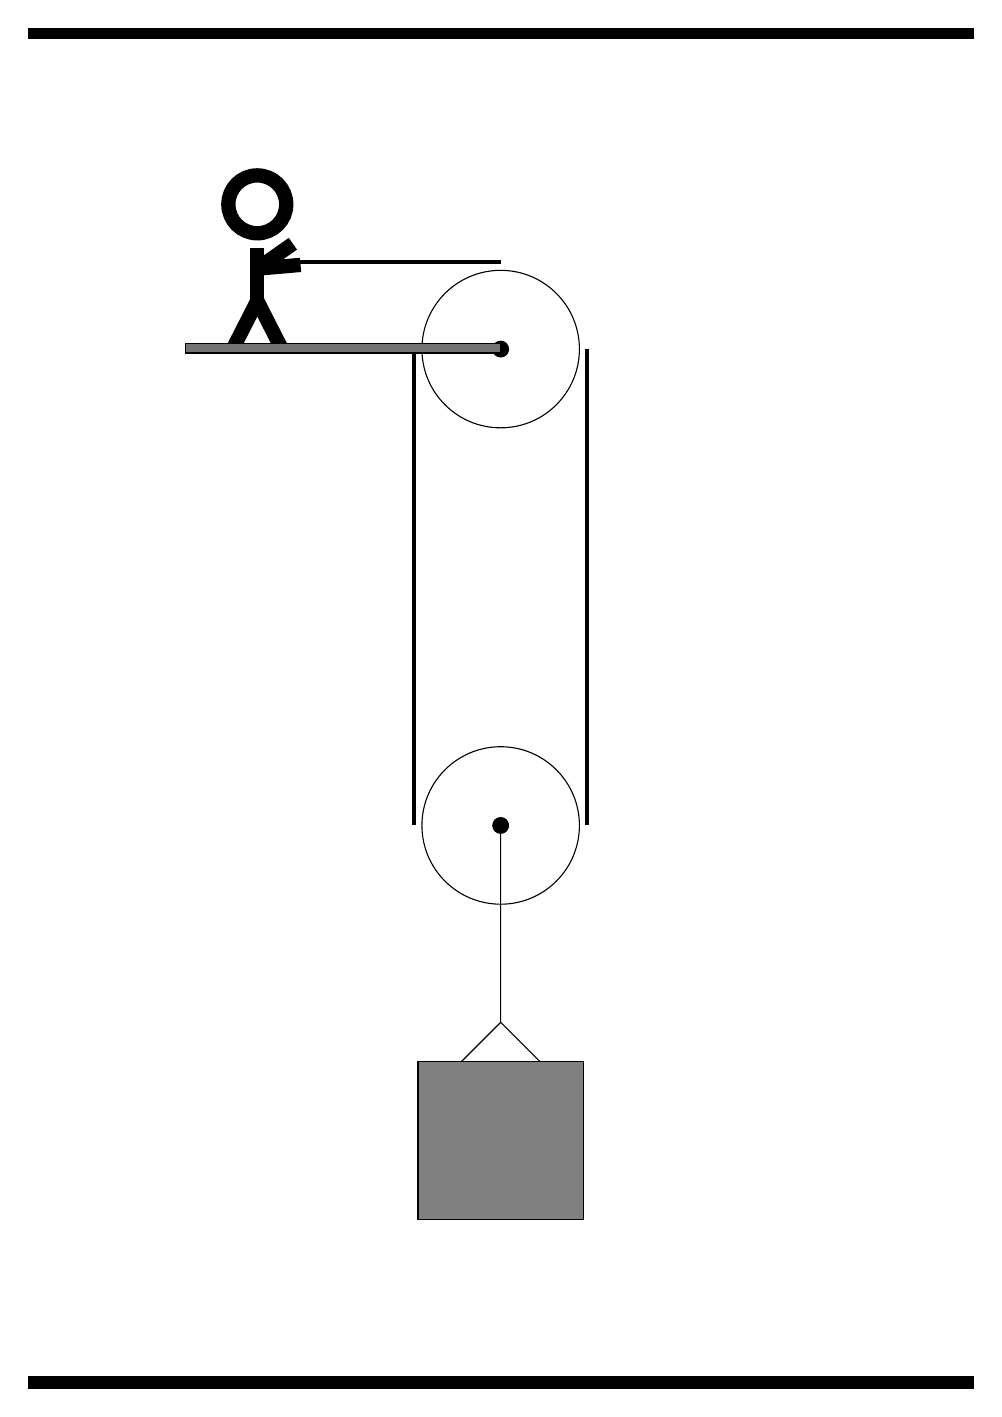
\begin{tikzpicture}
			%%%%% START %%%%%
			\draw[fill=black] (-4, 14) rectangle (8, 14.125);
			
			\draw (2, 4.0) circle (1);
			\draw[fill=black] (2, 4.0) circle (0.1);
			
			\draw (2, 10.05) circle (1);
			\draw[fill=black] (2, 10.05) circle (0.1);
			
			\draw (2, 4.0) -- (2, 1.5) -- (1.5, 1.0) -- (2.5, 1.0) -- (2, 1.5);
			\draw[fill=black!50] (0.95, 1.0) rectangle (3.05, -1.0);
			
			\draw[line width=0.5mm] (0.9, 10) -- (0.9, 4.0);
			\centerarc[line width=0.5mm](2, 4.0)(180:360:1.1);
			\draw[line width=0.5mm](3.1, 4.0) -- (3.1, 10.05);
			\centerarc[line width=0.5mm](2, 10.05)(0:90:1.1);
			\draw[line width=0.5mm](2, 11.15) -- (-1, 11.15);
			
			\node at (-1, 11.15) {\Strichmaxerl[10][-175][35]};
			\draw[fill=black!55] (-2, 10) rectangle (2, 10.125);
			
			\draw[fill=black] (-4, -3) rectangle (8, -3.15);
			%%%%% END %%%%%
		\end{tikzpicture}
	\end{figure}	
\end{document}